
\begin{ledgroupsized}[r]{120mm}
\footnotesize
\pstart
\noindent\textbf{Überlieferung:}
\pend
\end{ledgroupsized}
\begin{ledgroupsized}[r]{114mm}
\footnotesize
\pstart \parindent -6mm
\makebox[6mm][l]{\textit{L}}%
Aufzeichnung:
LH~XLII~5 Bl.~42. 
Ein Zettel (ca.~6,5~x~5~cm.);
linker, unterer und rechter Rand beschnitten.
Eine Seite auf Bl.~42~r\textsuperscript{o}; 
Rückseite nicht zugänglich, da der Zettel, zusammen mit LH~XLII 5 Bl.~41 und Bl.~43, 
auf einer leeren Seite von LH~XLII 5 Bl. 39\textendash40 aufgeklebt ist.
\pend
\end{ledgroupsized}
\selectlanguage{latin}
\vspace{8mm}
\pstart\noindent
\href{\Scan{LH_42_05_042r}}%
{\lbrack42~r\textsuperscript{o}\rbrack}\ 
\pend
\begin{edfigure}[1em][1em]    	%
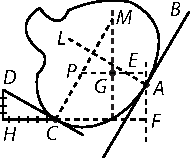
\includegraphics[scale=1]{gesamttex/edit_VIII-4/images/LH_42_05_042_d_042r.pdf}
\edcaption[0.5em]{%
\lbrack\textit{Fig.~1}\rbrack}
\end{edfigure}
\pstart
\noindent
Si 
\edtext{pondus\indexS{pondus} \textit{GAC}\lbrack,\rbrack}{%
\lemma{pondus}%
\Bfootnote{%
\textit{(1)}~\textit{G}
\textit{(2)}~\textit{GAC}
\textit{(a)}~\textit{L}}} 
cujus centrum gravitatis\indexS{centrum gravitatis} \textit{G}\lbrack,\rbrack\ incumbat duobus planis\indexS{pondus duobus planis incumbens} \textit{AB}, 
\edlabel{42_05_042_1a}%
\edtext{}{%
\xxref{42_05_042_1a}{42_05_042_1b}%
\lemma{\textit{CD}}%
\Bfootnote{%
\textit{(1)}~patet 
\textit{(2)}~\bracks{/} Ex punctis~\textit{L}}}%
\textit{CD} \lbrack\textit{Satz bricht ab}\rbrack.
\pend
\pstart
Ex punctis\edlabel{42_05_042_1b}
\textit{G} et \textit{C} demittantur 
\edtext{normales \textit{GE},}{%
\lemma{normales}%
\Bfootnote{%
\textit{(1)}~in
\textit{(2)}~\textit{GE},~\textit{L}}}
\textit{CF} in rectam horizonti\indexS{horizon} perpendicularem \textit{EF} transeuntem per \textit{A}. 
\edtext{Constat perinde esse ac si pondus\indexS{pondus} \textit{GCA} esset}{%
\lemma{Constat}%
\Bfootnote{%
\textit{(1)}~\textit{G} agere perinde ac si suspensum %
\textit{(2)}~perinde %
\textit{(a)}~esset %
\textit{(b)}~esse ac si pondus
\bars{\textit{GCA} \textit{erg.}}
\textit{(aa)}~suspensum ex \textit{G}, %
\textit{(bb)}~vel %
\textit{(cc)}~esset~\textit{L}}} 
suspensum ex puncto \textit{G} extremitate brachii \textit{GE} mobilis\indexS{brachium mobile} 
\edtext{circa \textit{E} quod vocemus pondus\indexS{pondus}}{%
\lemma{circa \textit{E}}%
\Bfootnote{%
\textit{(1)}~et ac %
\textit{(2)}~quod vocemus %
\textit{(a)}~punctu %
\textit{(b)}~pondus~\textit{L}}} 
\textit{G}, vel perinde esse ac si ex 
\edtext{puncto \textit{C} extremitate}{%
\lemma{puncto \textit{C}}%
\Bfootnote{%
\textit{(1)}~suspensum esset pondus quo %
\textit{(2)}~extremitate~\textit{L}}} 
brachii mobilis\indexS{brachium mobile} circa \textit{F} suspensum esset pondus\indexS{pondus} quod vocabimus pondus\indexS{pondus} \textit{C}, 
ita se habens ad pondus\indexS{pondus} \textit{G} ut \textit{GE} ad \textit{CF} seu reciproce ut brachia.\indexS{brachium}
Jam pondus\indexS{pondus} \textit{C} aget in planum\indexS{pondus agens in planum} 
\edtext{\bracks{\textit{CD}}}{%
\lemma{}%
\Bfootnote{\textit{C} \textit{L ändert Hrsg.}}}
potentia\indexS{potentia} quae sit ad totum pondus\indexS{pondus} \textit{C}, 
\edtext{ut \textit{DC} ad \textit{CH},}{%
\lemma{ut \textit{DC}}%
\Bfootnote{%
\textit{(1)}~ad \textit{CH} posito \textit{D} %
\textit{(2)}~cathetus ad %
\textit{(3)}~ad \textit{CH},~\textit{L}}} 
posito \textit{DH} 
\ledpb%
esse verticalem \textit{CH} horizontalem; ergo vis\indexS{vis quam patitur planum} quam patitur planum\indexS{planum}
\edtext{\textit{CD}}{%
\lemma{}%
\Bfootnote{%
\textit{CD} 
\textit{erg.~L}}}
est 
\edtext{ad pondus\indexS{pondus} \textit{G},}{%
\lemma{ad}%
\Bfootnote{%
\textit{(1)}~vim ponderis %
\textit{(2)}~pondus \textit{G}~\textit{L}}}
in ratione composita \textit{CH} ad \textit{DC}, et \textit{GE} 
\edtext{ad \textit{CF}. Jam $CH:DC\squaredots MG:\lbrack PM\rbrack$\lbrack,\rbrack\ fit}{%
\lemma{ad \textit{CF}}%
\Bfootnote{%
\textit{(1)}~seu in ratione $CH\cdot GE$ ad $DE\cdot CF$ \bars{seu \textit{streicht Hrsg.}} %
\textit{(2)}~. Jam $CH:DC\squaredots$ %
\textit{(a)}~$MP:GM$ %
\textit{(b)}~$MG:$ \bars{\textit{GP} \textit{ändert Hrsg.}} fit~\textit{L}}} 
ratio composita 
$MG\cdot GE:
\edtext{\lbrack PM\rbrack}{%
\lemma{}%
\Bfootnote{\textit{GP} \textit{L ändert Hrsg.}}}
\cdot CF$. 
\pend
